\chapter{绪论}\label{chap:introduction}

\section{课题研究背景}

\subsection{课题背景与意义}

随着移动网络技术和社交多媒体技术的快速发展与普及,人们能够越来越方便地通过网络在社交媒体上获取信息和交换意见。比如4G移动网络的普及以及5G移动网络的推进使得网络带宽不断增加,信息传输变得更加方便快捷。同时,诸如微信、微博、抖音、快手、斗鱼等热门社交媒体APP几乎成为人手必备的软件。因此,社交媒体和移动网络技术的发展极大地促进了用户生成式数据(User-Generated Content,UGC)的产生的传播\citep{pang-2013-unsupervised}。但是,海量的UGC数据使得人们难以从中快速找到自己感兴趣的内容。所以,人们希望引进某种技术来帮助人们快速、准确从海量数据中找到感兴趣的内容。例如,微博推出了热搜榜和话题榜来给用户呈现当前大多数人关注的热门话题,并取得不错的反馈。所以,以话题形式向人们呈现信息是一种有效的方式。基于此,产生了网络话题检测。网络话题检测通过对大规模的网络数据进行检测,将其中有意义的内容组织成网络话题,使得人们能够快速了解当前时事热点。

对于UGC数据,即用户生成内容数据,是指网站或其他开放性媒介的内容由其用户贡献生成。约2005年左右开始,互联网上的许多站点开始广泛使用用户生成内容的方式来提供服务。许多图片、视频、博客、论坛、社交、新闻类的网站都使用这种方式。随着互联网的发展,网络用户的交互作用得以体现。用户即是网络内容的创造者,也是网络内容的浏览者。每一个用户都可以生成自己的内容,互联网上的所有内容由用户创造,而不只是以前的某一些专业编辑。所以,互联网上的内容会飞速增长,形成一个多、广、专的局面。

对于网络话题,一般认为是针对某一现实事件的相关报道和言论的集合。围绕某一个话题的报道、言论和观点在网络上迅速传播扩散,能够在短时间、大范围内形成具有强大影响力的网络舆情。比如,针对当下热门的“奔驰女车主维权”事件是一个话题。当该事件在网络上曝光后,所有与“奔驰女车主维权”相关的信息——记者报道、用户评论、官方回应等与之相关的内容,都是该话题的组成部分。该话题在短时间被大量传播浏览,引起一片声讨,使得政府及其有关部门立刻着手调查。同时,随着该话题不断被传播,逐渐引出一系列相关话题——“奔驰金融服务费”、“奔驰排放测试涉嫌造假”等。这大量的话题中包含了许多用户特有的行为数据,利用这些数据,可以挖掘用户的行为习惯和偏好,从而为用户构建用户画像。对于商业公司,可以利用构建的用户画像为用户推荐商品和广告;对于政府,可以用于舆情监控、敏感信息监管等途径。因此,如何快速准确地从大规模网络数据中检测热门话题是一项非常具有现实意义和研究价值的工作。

\subsection{研究问题与难点}

传统的话题检测和追踪任务(Topic Detection and Tracking,TDT)\citep{allan-1998-TDT}致力于将每篇新闻文档分配到至少一个话题中。具体地讲,TDT是从经过专业编辑的新闻文档中生成话题\citep{Allan2002Topic}。而这些经过专业编辑的文档与网络数据有着极大的不同。

\textbf{网络数据的特点:}
\begin{enumerate}
    \item[(1)] 规模大

    任何人都可以通过网络在社交媒体上创作,且社交媒体对用户在其上发表的内容并没有太多的约束。再加上这些年快速发展的网络技术以及多媒体技术,极大地促进了网络数据的产生和传播,使得网络数据的规模越来越庞大;

    \item[(2)] 约束少

    网络数据由用户在社交媒体上创作产生,而社交媒体对这些创作内容并没进行格式和内容上的约束。导致网络数据受到较少的约束。

    \item[(3)] 噪声多

    网络数据具有很多噪声,即与主题无关的文本和图像等信息。大部分网络数据是由普通用户创作,相比专业编辑,普通用户在创作时都是很随意的。导致网络数据存在较多的噪声。

    \item[(4)] 稀疏

    组成网络数据的文本和视觉信息通常是简短的,在用特征表示的时候就会非常稀疏。
\end{enumerate}

所以网络话题检测要处理的是大规模的网络数据,并且这些数据往往是简短的、稀疏的和充满噪声的\citep{wxzhao2011comparing}。与此同时,这大规模的网络数据中却只有很少一部分能够被组织成热点话题,大概只有5\%的数据能被组织成热点话题\citep{pang-2013-unsupervised}。也就是说网络数据中还存在着大量的噪声数据。因此,网络话题检测不仅面临着大规模的数据、低效的特征,也面临着大量的噪声。这使得传统的话题检测算法\citep{yang1998astudy,Allan2002Topic,zhai2005tracking,ponsporrata2007topics}不再适合处理网络数据。

一个直观的方法是在噪声存在的情况下对网络数据进行聚类。然而海量的噪声使得能够处理少量噪声的聚类算法\citep{bojchevski2017RSC,maurus2016skinny,blei-2003-LDA}也不再奏效。除了网络数据外,网络话题的相应特点也会对网络话题检测带来挑战。

\textbf{网络话题特点:}
\begin{enumerate}
    \item[(1)] 大小不确定

    由于每个用户对于话题有不同认识,所以很难界定一个话题的大小。有的人认为强相关的数据才能构成话题,而有的人认为弱相关的数据也能构成话题。比如针对“奔驰女车主维权”的报道和“奔驰金融服务费”报道,有的人认为这是同一个话题,因为都是由奔驰车引出的一系列事件。而有的人却认为这两个报道的主要内容不一样,所以不是同个话题。因此,我们无法找到一种通用的方法来确定话题的大小;

    \item[(2)] 数量不确定性

    正是由于话题的多粒度性,导致不能确定一个话题的大小,从而不能确定话题的数量。而且在一个大规模的网络数据集中,我们也不可能提前明确知道话题的数量。
\end{enumerate}

所以我们在解决大规模网络话题检测的时候,不仅要考虑到网络数据的特点,也要考虑到网络话题的特点。综上,针对课题研究方向,我们主要解决以下几个问题:
\begin{enumerate}
    \item[(1)] 大规模的网络数据带来的话题检测效率低下的问题;
    \item[(2)] 高噪声的网络数据带来的话题检测效果差的问题;
    \item[(3)] 稀疏特征带来的低效特征问题;
    \item[(4)] 话题大小不确定性问题;
    \item[(5)] 话题数量不确定性问题;
\end{enumerate}



\section{常用数据集}

在话题检测领域,MCG-WEBV\citep{cao-2009-mcg}和YKS\citep{zhang2013cross}是两个常用的数据集。许多网络话题检测算法使用这两个数据集来验证算法的性能。表\ref{tab:dataset}汇总了这两个数据集的基本信息。
\begin{table}[!htbp]
    \caption{MCG和YKS数据集的基本情况汇总}
    \label{tab:dataset}
    \centering
    % \footnotesize% fontsize
    % \setlength{\tabcolsep}{4pt}% column separation
    % \renewcommand{\arraystretch}{1.2}%row space
    \begin{tabular}{|p{2.35cm}<{\centering}|p{1cm}<{\centering}|p{1cm}<{\centering}|p{2.5cm}<{\centering}|p{1cm}<{\centering}|p{3cm}<{\centering}|}
        \hline
        数据集 & 话题数量 & 网页数量 & 所有话题包含网页数 & 词典规模 & 平均每个网页包含词语数量\\
        %\cline{2-9}% partial hline from column i to column j
        \hline
        \hline
        MCG-WEBV & $73$ & $3660$ & $832$ & $9212$ & $35$\\
        \hline
        YKS & $298$ & $8660$ & $990$ & $80294$ & $228$\\
        \hline
    \end{tabular}
\end{table}

\subsection{MCG-WEBV}
MCG-WEBV数据集爬取了YouTube自2008年12月到2009年2月间的“浏览最多”的视频,包含了15类。同时还爬取了与这些视频相关的视频以及相同作者上传的视频。最终MCG-WEBV包含了80031个视频。

除了视频数据外,MCG-WEBV还包含丰富的信息:
\begin{itemize}
	\item 5种元特征:视频ID、上传用户名、上传时间、视频长度、视频类别;
	\item 人工分类的15类视频类别及其标签;
	\item 8种网页特征:标题、描述、标注、评级、评论数、拍摄张数等;
	\item 9种视觉特征:166维颜色直方图特征、320维边缘直方图特征等;
	\item 采用文本特征模型产生的文本特征和36维的音频特征;
\end{itemize}

MCG-WEBV对核心数据集进行了人工标注,最终得到73个话题。这些话题由话题热度决定。而话题热度主要与话题关注度和持续时间相关。在MCG-WEBV中,话题的关注度由话题包含的视频数和视频点击数决定,话题的持续时间为话题中第一个视频的上传时间与用户最后观看时间之间的间隔。所以,话题的热度由公式\ref{eq:hottopic}决定。其中$\tau(t)$指话题$t$的持续时间,$N(t)$表示话题$t$的视频总数,$V(t)$表示话题$t$中视频被观看的次数。
\begin{equation}\label{eq:hottopic}
H(t) = \log\frac{|N(t)|*|V(t)|}{\tau(t)}
\end{equation}

对于热门话题的标注,主要分为以下三个步骤:
\begin{enumerate}
    \item[(1)] 对每个视频提取标题和标注来构建特征向量,然后通$k$均值聚类算法对特征向量进行无监督聚类,总共得到113个候选话题;
    \item[(2)] 通过人工对这113个候选话题进行筛选,删除话题内无关的视频,对每个话题提供简单的描述;
    \item[(3)] 对筛选结果进行后处理,剔除持续时间短、网页少的的话题,融合语义相近的话题,最终得到73个人工标注的网络话题 。
\end{enumerate}

\subsection{YKS}

YKS是一个跨媒体的多模态数据集。主要由优酷网$\footnote{https://www.youku.com/}$的视频数据和新浪网$\footnote{https://www.sina.com.cn/}$的新闻数据共同组成。其中,约有75\%的数据只包含文本信息,约有25\%的数据同时包含文本信息和视觉信息。此外还有极少量的数据只包含视觉信息。

对于优酷视频,逐日爬取了从2012年5月1号开始的视频点击率在5万以上的视频,总共得到5500多个视频。然后经过过滤、剔除长度小于5秒和大于1小时的视频,最终得到2131个视频数据。除了视频外,还有其他相关的数据,比如视频标题、视频标注、视频描述、视频点击率、上传时间等。

对于新浪网的新闻数据,爬取了从2012年5月1号到2012年5月31号的新浪网发布的所有新闻。包括新闻标题、新闻正文(文本、图像、视频)和其他辅助信息,比如新闻发布时间、新闻标签、新闻点击率、新闻相关链接等。总共有30000多篇新闻文档,经过过滤空白新闻、纯图像新闻、纯视频新闻等处理后,最终剩余7325篇新闻文档。

YKS数据集同样经过话题的人工标注。在YKS数据集中,总共标注了318个话题,其中225个话题只包含新浪新闻的纯新闻,20个话题只包含优酷网的纯视频,另外73个话题同时包含新浪新闻和优酷视频。人工标注主要为一下三个步骤:
对于热门话题的标注,主要分为以下三个步骤:
\begin{enumerate}
    \item[(1)] 提取新闻或视频的文本特征,使用词袋模型表示成特征向量。然后计算特征向量之间的余弦距离;
    \item[(2)] 使用$k$均值聚类算法对这些特征向量进行无监督聚类,总共得到400个候选话题;
    \item[(3)] 对400个候选话题进行人工标注,删除话题中噪声数据,合并较小的话题以及拆分较大的话题。
\end{enumerate}

经过人工标注后,过滤掉网页个数小于4的话题。最终得到318个人工标注的网络话题,同时为每个网络话题提供了简单的描述和代表性的单词。



\section{论文内容与组织结构}

本文的整体结构如图 \ref{fig:mainstructure}所示,主要由以下五个部分组成:

第一章绪论:介绍了课题研究背景、常用数据集和论文内容与组织结构。其中课题研究背景包括课题研究的背景与意义以及主要解决的难点问题。常用数据集详细介绍了网络话题检测中常用的两个数据集。论文内容与组织结构介绍了本文的主要内容以及结构框架。

第二章介绍了目前话题检测领域的国内外研究现状和存在的问题。同时简要介绍了本论文给出的解决方案。

第三章针对网络话题生成部分,我们提出了新的无模型、无需复杂参数优化的算法来达到快速生成网络话题的目的。然后在两个数据集上使用多种评测标准对比我们提出的算法和当前最好的算法。

第四章针对网络话题排序部分,我们改进了原来的泊松去卷积算法,提出了一种可扩展性的随机泊松去卷积算法。该算法能够高效地处理大规模的网络数据。然后,我们构造了一个较大规模的人工数据集来验证我们算法的收敛速度。同时,我们还实现了该算法的异步并行版本,并在数据集上经验地验证其是有效的。

第五章对本文提出两个部分的工作进行总结,根据当前网络话题检测领域所出现的新特点和新问题,对下一步的研究计划进行了展望。
\begin{figure}[!htbp]
    \centering
    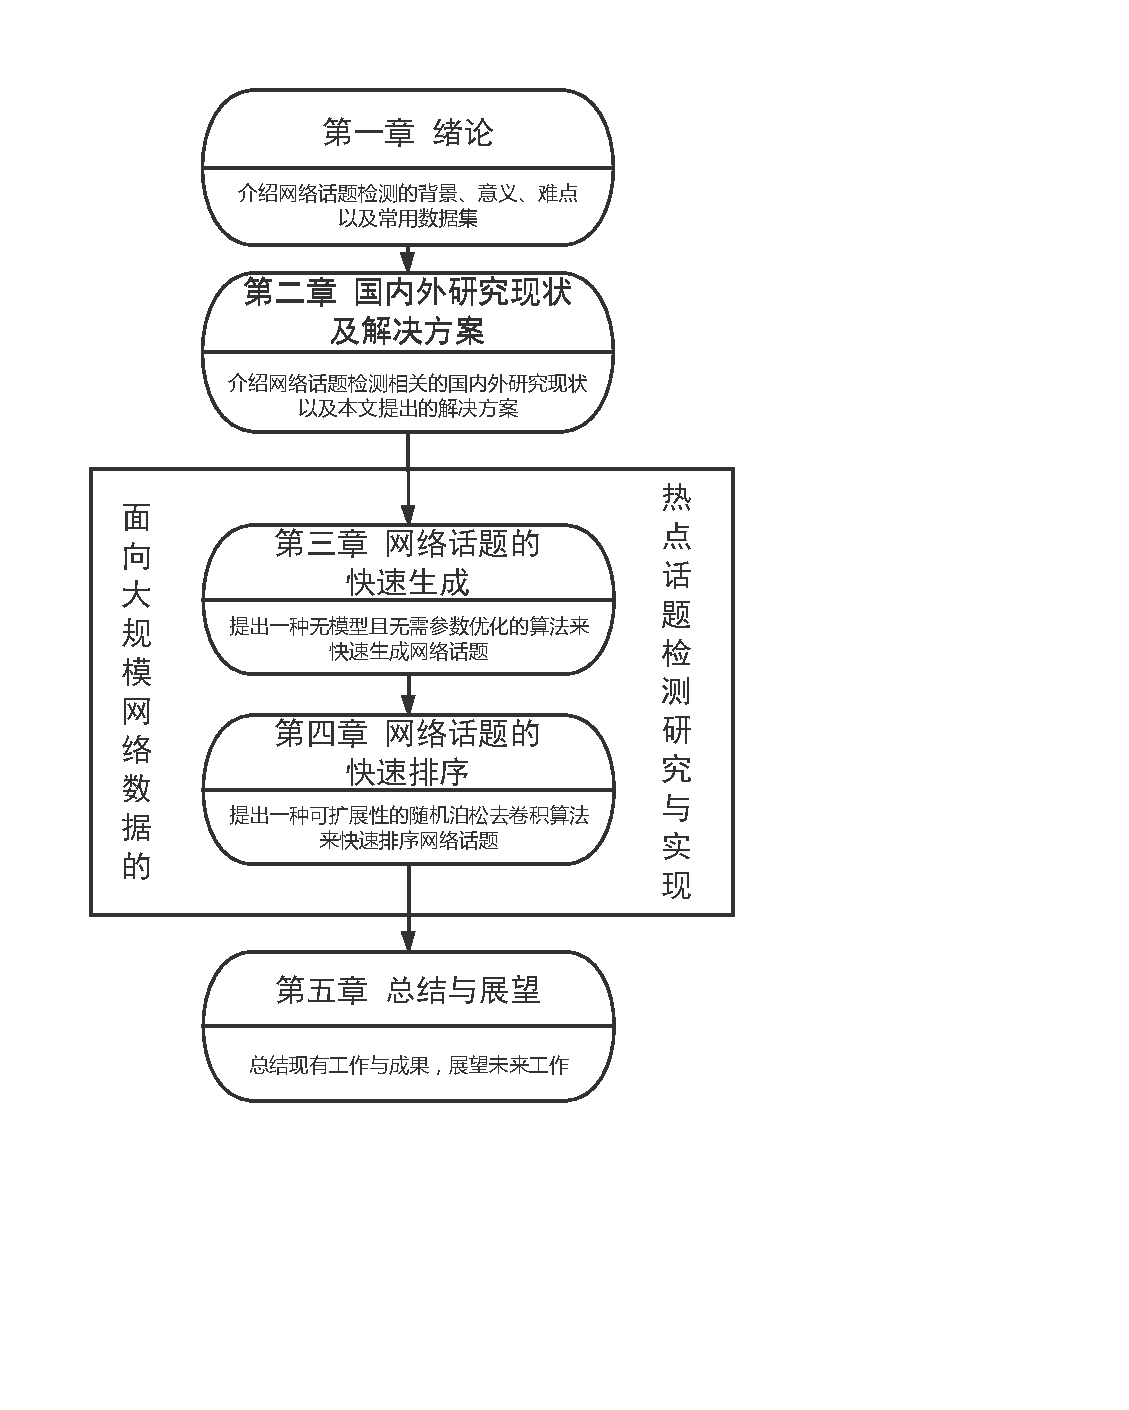
\includegraphics[width=0.70\textwidth]{mainstructure}
    \caption{论文总体结构}
    \label{fig:mainstructure}
\end{figure} 